%\VignetteIndexEntry{Using PING with paired-end sequencing data}
%\VignetteDepends{PING,parallel}
%\VignetteKeywords{Preprocessing, ChIP-Seq, Sequencing}
%\VignettePackage{PING}
\documentclass[11pt]{article}
%\usepackage{hyperref}
\usepackage{url}
\usepackage{color, pdfcolmk}
\usepackage{underscore}
\usepackage[authoryear,round]{natbib}
\bibliographystyle{plainnat}
 %Introduce newlines automatically in R code


\newcommand{\scscst}{\scriptscriptstyle}
\newcommand{\scst}{\scriptstyle}

\author{Xuekui Zhang\footnote{ubcxzhang@gmail.com}, Sangsoon
Woo\footnote{swoo@fhcrc.org}, Raphael Gottardo\footnote{rgottard@fhcrc.org} and
Renan Sauteraud\footnote{rsautera@fhcrc.org}}

\usepackage{Sweave}
\begin{document}
%To display nice multilines chunks of code

\title{PING: Probabilistic Inference for Nucleosome Positioning with MNase-based or Sonicated Short-read Data.}
\maketitle



\textnormal {\normalfont}
This vignette presents a workflow to use PING on paired-end sequencing data.

\tableofcontents
%%%%%%%%%%%%%%%%%%%%%%%%%%%%%%%%%%%%%%%%%%%%%%%%%%%%%%%%%%%%%%%%%%%%%%%%%%%%%%%
\newpage


\section{Licensing and citing}

Under the Artistic License 2.0, you are free to use and redistribute this software. 

If you use this package for a publication, we would ask you to cite the following: 

\begin{itemize}
\item[] Xuekui Zhang, Gordon Robertson, Sangsoon Woo, Brad G. Hoffman, and Raphael Gottardo. (2012). Probabilistic Inference for Nucleosome Positioning with MNase-based or Sonicated Short-read Data. PLoS ONE 7(2): e32095.
\end{itemize}


\section{Introduction}
For an introduction to the biological background and PING method, please refer to the PING user guide.


\section{PING analysis steps}
A typical PING analysis consists of the following steps:
\begin{enumerate}
  \item Extract reads and chromosomes from bam files.
  \item Segment the genome into candidate regions that have sufficient aligned reads via `segmentPING'
  \item Estimate nucleosome positions and other parameters with PING
  \item Post-process PING predictions to correct certain predictions
\end{enumerate}

As with any R package, you should first load it with the following command:

\begin{Schunk}
\begin{Sinput}
> library(PING)
\end{Sinput}
\end{Schunk}

\section{Data Input and Formatting}
In order to use the PE version of PING, the input has to be slightly different.
Instead of a GRanges object, the new segmentation method use a list of reads and
a chromosome.

%From a bed file, you can create such a list manually by first reading the file
%using read.table, then assigning the resulting data.frame to the 'P' attribute
%of a list. If some reads are missing an end or a start coordinate, they can
%still be used. The reads with a missing start are treated as reverse reads and
%should be assigned to an attribute 'yRm' to the same list. Reads with a missing
%end are treated as Forward reads and have to be assigned to an attribute 'yFm'.

The package comes with a function to convert bam files into the appropriate
list. We provide a small bam file with two chromosomes of the yeast to be used
as an example in this vignette.

\begin{Schunk}
\begin{Sinput}
> yeastBam <- system.file("extdata/yeastChrI_M.bam", package = "PING")
\end{Sinput}
\end{Schunk}

Bam files can be huge, therefore, the default behaviour is to save the resulting
R objects on disk with one file per chromosome.

\begin{Schunk}
\begin{Sinput}
> prePING(bamFile = yeastBam, outpath = "./")
\end{Sinput}
\end{Schunk}
This will create one file for each chromosome found in `micro.bam' in the curent
folder. Then, the files can be loaded separately in order to use the
segmentation function.

If the bam file is small enough that it can be handled by the computer's memory,
it is possible to return a list of lists to be used as input. 
\begin{Schunk}
\begin{Sinput}
> inputList <- prePING(bamFile = yeastBam, save = FALSE)
\end{Sinput}
\begin{Soutput}
[1] "chrI"
[1] "chrM"
\end{Soutput}
\end{Schunk}
$inputList$ has one attribute per chromosome, here `chrI' and `chrM'.


\section{PING analysis}

\subsection{Genome segmentation}
PING is used the same way for paired-end and single-end sequencing data. The
function \texttt{segmentPING} will decide which segmentation method should be
used based on the data type. 
When dealing with paired-end data, four new arguments have to be passed to the
function: a chromosome chr and three parameters used in candidate region
selection: islandDepth, min_cut and max_cut.

These arguments control the size and required coverage for a region to be
considered as a candidate.

In order to improve the computational efficiency of the PING package, if you
have access to multiple cores we recommend that you do parallel computations via
the \texttt{parallel} package. In what follows, we assume that \texttt{parallel}
is installed on your machine. If it is not, you could omit the first line, and
calculations will occur on a single CPU. By default the command is not run. Note
that the \texttt{segmentPING} and \texttt{PING} functions will automatically
detect whether you have initialized a cluster and will use it if you have.

\begin{Schunk}
\begin{Sinput}
> library(parallel)
\end{Sinput}
\end{Schunk}


\begin{Schunk}
\begin{Sinput}
> segPE <- segmentPING(inputList$chrM, chr = "chrM", islandDepth = 3, 
     min_cut = 50, max_cut = 1000)
\end{Sinput}
\end{Schunk}

It returns a \texttt{segReadsListPE} object.


\subsection{Parameter estimation}
The only difference when using \texttt{PING} for paired-end data is the argument PE that has to be set to TRUE.

%paraP<-setParaPriorPING(xi=150, rho=1.2, alpha=12, beta=20000, lambda=-0.000064, dMu=200)
\begin{Schunk}
\begin{Sinput}
> ping <- PING(segPE, PE = TRUE)
\end{Sinput}
\end{Schunk}
The returned object is of class pingList and can be post-processed.


\section{Post-processing PING results}
Here again, we set the argument PE to TRUE, and use postPING normally.

\begin{Schunk}
\begin{Sinput}
> {
     sigmaB2 = 3600
     rho2 = 15
     alpha2 = 98
     beta2 = 2e+05
 }
> PS = postPING(ping, segPE, rho2 = rho2, alpha2 = alpha2, beta2 = beta2, 
     sigmaB2 = sigmaB2, PE = TRUE)
\end{Sinput}
\begin{Soutput}
 The 6 Regions with following IDs are reprocessed for singularity problem: 
(0.773,114]80   (114,228]39   (114,228]51   (114,228]79   (114,228]82 
           80           153           165           193           196 
 (114,228]106 
          220 

 The 17 Regions with following IDs are reprocessed for atypical delta: 
[1] 155 190 129  41  37  28
[1] "No predictions with atypical sigma"

 The 172 regions with following IDs are reprocessed for Boundary problems: 
[1]  4  6  7 12 18 20
\end{Soutput}
\end{Schunk}
The result output $PS$ is a dataframe that contains estimated parameters of each nucleosome, users can use write.table command to export the selected columns of the result.
\begin{Schunk}
\begin{Sinput}
> head(PS)
\end{Sinput}
\begin{Soutput}
     ID  chr         w         mu    delta  sigmaSqF  sigmaSqR        se
96   32 chrM 0.3593627 11633.3048 119.5366  876.2446  925.5663 12.894380
518 163 chrM 0.6357604 63067.6607 139.9552 1377.8030 1047.7658  5.252400
1     1 chrM 0.5649540   334.6209 135.6721 1224.5633 1536.3315  8.075665
62   21 chrM 0.3226948  7231.8196 171.9921 1509.9668 1268.8164 10.375752
700 228 chrM 0.3263701 84916.4188 149.8338  955.7443 1378.1164  8.668972
524 164 chrM 0.4261601 64274.6381 141.5827 2071.6632 1815.6545 13.725905
        score   scoreF   scoreR minRange maxRange      seF       seR rank
96  1328347.9 685598.9 642749.0    11290    12500 15.98384 11.486267    1
518 1141956.1 570978.1 570978.1    62728    63762  7.37211  6.219118    2
1   1042681.7 557049.1 485632.6      187      949  9.26240  9.202644    3
62  1014115.0 442782.6 571332.4     6838     8133 11.68977 11.680681    4
700 1013486.1 585252.5 428233.6    84565    85803 11.57234  9.151415    5
524  984937.2 413959.1 570978.1    63281    64582 15.56970 14.943394    6
\end{Soutput}
\end{Schunk}

\section{Using the results}
\texttt{PING} comes with a set of tools to export or visualize the prediction.
Here, we only show how to export the results into bed format for further use
and how to make a quick plot to summarize the prediction. For more information
on how to export the results or make more complex plots, refer to the section
`Result output' of PING vignette.

The function \texttt{makeRangedDataOutput} offers a simple way to convert the
prediction results into a \texttt{RangedData} object ready to be exported with
the package \texttt{rtracklayer}.

\begin{Schunk}
\begin{Sinput}
> rdBed <- makeRangedDataOutput(PS, type = "bed")
> library(rtracklayer)
> export(rdBed, "nucPrediction.bed")
\end{Sinput}
\end{Schunk}

The exported file contain all the predicted nucleosomes displayed in bed format
and ranked by score.

\vspace{10pt}
The function \texttt{plotSummary} will generate a plot displaying the coverage
by the reads used as input and the predicted position of the
nucleosomes of $PS$ for the given ranges.

\begin{Schunk}
\begin{Sinput}
> plotSummary(PS, inputList$chrM, chr = "chrM", from = 1000, to = 4000)
\end{Sinput}
\end{Schunk}
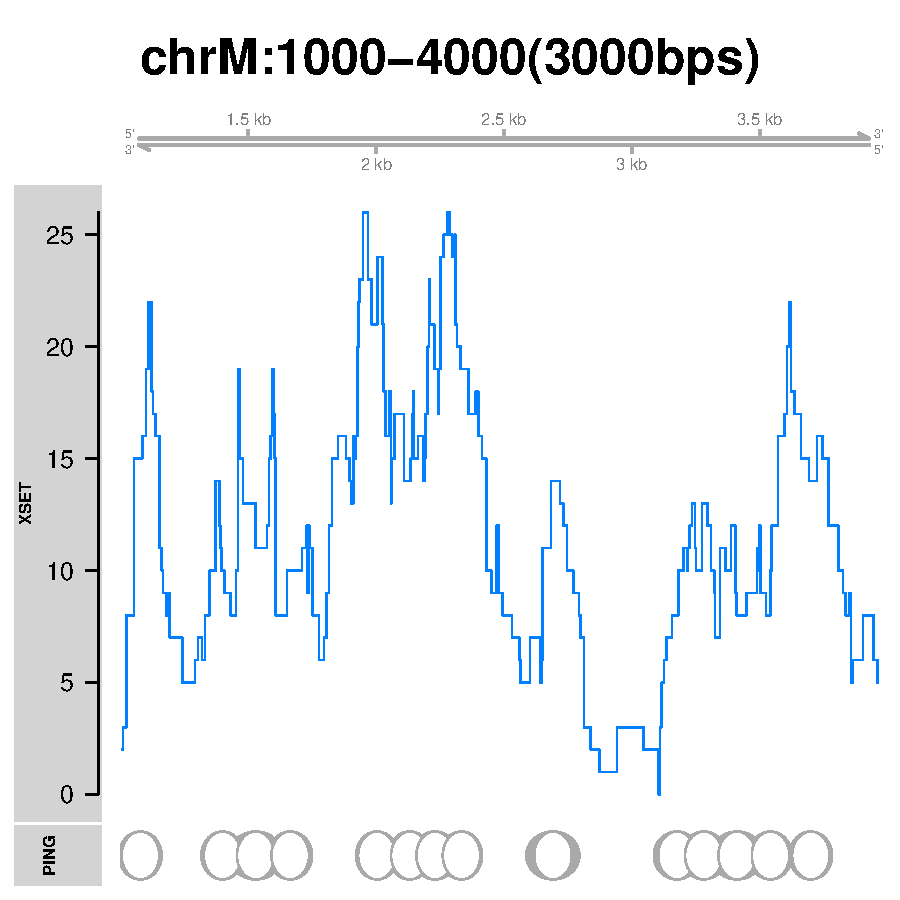
\includegraphics{PING-PE-plotSummary}

\end{document}

